\subsection{Perceptron}

\begin{frame}
\frametitle{Perceptron}

\begin{columns}

\column{0.45\textwidth}
\begin{itemize}
\item Ähnliche Aktivierungsfunktion wie beim MP-Neuron
\item Jedoch gewichtete Eingabewerte
\end{itemize}


\column{0.4\textwidth}
\begin{figure}
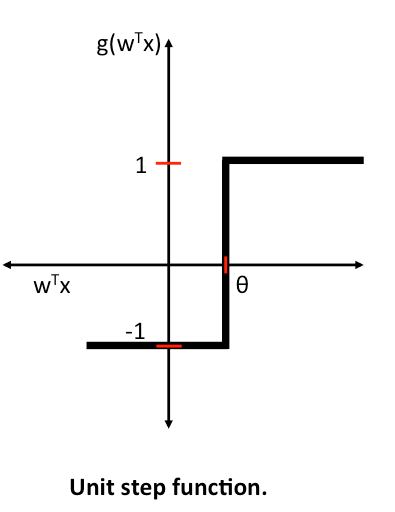
\includegraphics[width=.8\linewidth]{./geschichtliches/perceptron/img/perceptron_einheitsSprungfunktion_alpha}
\end{figure}

\end{columns}


\hspace{1mm}
\hrule


\begin{columns}

\column{0.4\textwidth}
\begin{align*} 
\mathbf{w} = \begin{bmatrix}
    w_{1}  \\
    \vdots \\
    w_{m}
\end{bmatrix}
\quad  \mathbf{x} = \begin{bmatrix}
    x_{1}  \\
    \vdots \\
    x_{m}
\end{bmatrix}
\end{align*}

\column{0.4\textwidth}
\begin{align*}
\begin{split}
z & =  w_1x_{1} + \dots + w_mx_{m} \\
 & = \sum_{j=1}^{m} x_{j}w_{j} \\
 & = \mathbf{w}^T\mathbf{x}
\end{split}
\end{align*}
\end{columns}

\note[item]{1958: US-amerikanische Psychologe / Informatiker Frank Rosenblatt}
\note[item]{älteste heutzutage noch genutzte NN}
\note[item]{inspiriert vom Auge einer Fliege
\begin{itemize}
    \item Flugrichtung - Entscheidungen teils direkt im Auge getroffen
\end{itemize}}

\note[item]{Weiterentwicklung der MP-Zelle}
\note[item]{Eingabewerte mit Gewichten priorisiert
\begin{itemize}
    \item Auf Formel verweisen
\end{itemize}}

\note[item]{Gleich bleibt jedoch die binäre Klassifikation
\begin{itemize}
    \item Verweis auf Unit step function
    \item hier jedoch nicht Wahrheitswerte sondern -1 und 1
\end{itemize}}

\end{frame}


\begin{frame}
\frametitle{Aufbau}

\begin{figure}
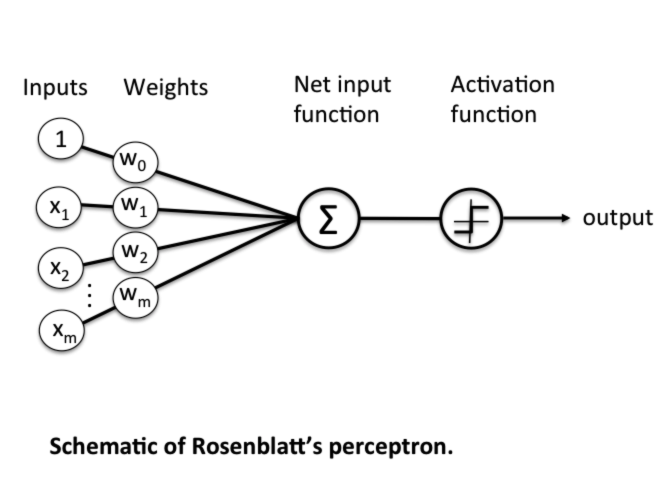
\includegraphics[width=.6\linewidth]{./geschichtliches/perceptron/img/perceptron_schematisch_alpha}
\end{figure}

\hrule


\begin{columns}

\column{0.4\textwidth}
\begin{align*}
g(z) =\begin{cases}
    1 & \mbox{if } z \geq 0 \\
	-1 & \mbox{if } z < 0 
  \end{cases}
\end{align*}
\vspace{1mm}

\column{0.4\textwidth}
\begin{align*}
\begin{split}
z & = \mathbf{w_0x_{0}} + w_1x_{1} + \dots + w_mx_{m} \\
 & = \sum_{j=0}^{m} x_{j}w_{j} \\
 & = w^Tx
\end{split}
\end{align*}

\end{columns}


\note[item]{Grafik erläutern}
\note[item]{Konvention: 
\begin{itemize}
    \item erleichtert später Notation der Lernregel
    \item Schwellwert auf andere Seite der z-Wert Gleichung ziehen
\end{itemize}}

\end{frame}


\begin{frame}
\frametitle{Lernregel - Ablauf}

\begin{itemize}
\item Modell übernimmt selbst die Anpassung der Gewichte
\item Test mittels einer Menge von gelabelten Trainingsdatensätzen
\end{itemize}
\hspace{1mm}

\begin{block}{Grober Ablauf}
\begin{itemize}
\item Initialisiere die Gewichte mit einem sehr kleinen Wert oder 0.
\item Für jeden Datensatz der Menge von Trainingsdatensätzen:
\begin{itemize}
	\item Berechne den Ausgabewert des Systems
	\item Gleiche die Gewichte an
\end{itemize}
\end{itemize}
\end{block}

\note[item]{Rosenblatt erfindet \emph{lernenden} Algorithmus}
\note[item]{Auf Menge von Trainingsdatensätzen zurückgegriffen
\begin{itemize}
    \item Datensätze bestehen aus Ein- und erwarteten Ausgabewerten
    \item in Literatur auch \emph{gelabelte} Werte genannt
\end{itemize}}

\note[item]{Lernalgorithmus - grobe Zusammenfassung
\begin{itemize}
    \item Gewichte mit kleinem Wert / 0 vorinitialisieren
    \item Datensätze durchiterieren
    \begin{itemize}
        \item Ausgabewert berechnen
        \item Gewichte angleichen
    \end{itemize}
\end{itemize}}

\end{frame}


\begin{frame}
\frametitle{Lernregel - Formel}

\begin{block}{Angleichung der Gewichte}
\begin{itemize}
\item Gewichte komponentenweise angleichen: $w_j := w_j + \Delta w_j$
\item Gewichtsänderung: $\Delta w_j = \eta \; (\text{target}^{(i)} - \text{output}^{(i)})\;x^{(i)}_{j}$
\end{itemize}
\end{block}

\begin{itemize}
\item Beispiel - Iteration mit zweidimensionalem Trainingsvektor:
\begin{align*}
\begin{aligned}
& \Delta w_0 = \eta(\text{target}^{(i)} - \text{output}^{(i)}) \\
& \Delta w_1 = \eta(\text{target}^{(i)} - \text{output}^{(i)})\;x^{(i)}_{1} \\
& \Delta w_2 = \eta(\text{target}^{(i)} - \text{output}^{(i)})\;x^{(i)}_{2}
\end{aligned}
\end{align*}
\end{itemize}

\note[item]{Erste Formel auf Slide beschreiben
\begin{itemize}
    \item Gewichte können zu Gewichtsvektor zusammengezogen werden 
    \begin{itemize}
        \item hier komponentenweise betrachtet
    \end{itemize}
    \item Delta (Dreieck) wird stets als Änderung verstanden
\end{itemize}}

\note[item]{Exponent \emph{i} hierbei jeweils als Index des Trainingsvektors in Menge}
\note[item]{Lernalgorithmus arbeitet inkrementell
\begin{itemize}
    \item Lernrate (eta) bestimmt wie stark die Gewichte pro Durchlauf angeglichen werden
    \item Differenz mit Lernrate und Eingabewert multipliziert
\end{itemize}}

\note[item]{Iteration mit 2d - Eingabevektor
\begin{itemize}
    \item w0 hierbei der Schwellwert selbst
    \item Faktor x weggelassen da bereits gleich 1
    \item Nutzung der beschriebenen Notation
\end{itemize}}

\end{frame}


\begin{frame}
\frametitle{Lernregel - Trainingsbeispiele}

\begin{block}{Gewichtsänderung}
$\Delta w_j = \eta \; (\text{target}^{(i)} - \text{output}^{(i)})\;x^{(i)}_{j}$
\end{block}

\begin{itemize}
\item Trainingsdatensatz richtig erkannt: 
\begin{align*}
\begin{aligned}
& \Delta w_j = \eta \big( (-1^{(i)}) - (-1^{(i)}) \big)\;x^{(i)}_{j} = 0 \\
& \Delta w_j = \eta(1^{(i)} - 1^{(i)})\;x^{(i)}_{j} = 0 \\
\end{aligned}
\end{align*}

\item Trainingsdatensatz falsch erkannt:
\begin{align*}
\begin{aligned}
& \Delta w_j = \eta \big( 1^{(i)} - (-1^{(i)}) \big) \;x^{(i)}_{j} = \eta(2)\;x^{(i)}_{j} \\
& \Delta w_j = \eta \big( (-1^{(i)}) - 1^{(i)} \big) \;x^{(i)}_{j} = \eta(-2)\;x^{(i)}_{j} \\
\end{aligned}
\end{align*}

\end{itemize}

\note[item]{Erinnerung: erst target dann output}
\note[item]{Richtig erkannt
\begin{itemize}
    \item Generell Ausgabe 0, keine Änderung
    \item Beide Falsch: -1
    \item Beide Richtig: +1
\end{itemize}}

\note[item]{Falsch erkannt
\begin{itemize}
    \item output zu klein
    \begin{itemize}
        \item erwartetet +1 bekommen -1 
        \item Positiver (Differenz-)Faktor 
    \end{itemize}

    \item output zu groß
    \begin{itemize}
        \item erwartetet -1 bekommen +1 
        \item Negativer (Differen-)Faktor
    \end{itemize}
\end{itemize}}

\end{frame}


